\documentclass[conference]{IEEEtran}

\usepackage{cite}
\usepackage{graphicx}
\usepackage{amsmath}
\usepackage{amssymb}
\usepackage{multirow}
\usepackage{array}
\usepackage{url}
\usepackage{float}
\usepackage{booktabs}
\usepackage[ruled,vlined]{algorithm2e}
\usepackage[caption=false,font=footnotesize]{subfig}
\usepackage{tikz}
\usepackage{makecell}

% =====================================================================
% NOTE TO AUTHORS (v4):
% v4 aligns the paper with the actual training code:
%   - stage-specific loss formulations (plain MSE for Stages 1/2;
%     weighted physical loss + L2-to-init for Stage 3),
%   - mask-projection input acknowledged in the architecture,
%   - corrected residual-block description (no LayerNorm, dropout 0.1),
%   - hyperparameter table now stage-structured and reflects argparse
%     defaults that were used during training.
% Multi-seed evaluation and a plain-MLP baseline remain explicitly
% deferred to the journal extension (acknowledged in Sec. IV.A and
% Limitations).
% =====================================================================

\begin{document}

\title{Learning and Transfer of Robot Forward Kinematics Across Varying Degrees of Freedom}

\author{
\IEEEauthorblockN{Chissanupong Saengsint}
\IEEEauthorblockA{
School of Engineering\\
University of Birmingham\\
Birmingham, United Kingdom\\
Email: chissanupong.sae@gmail.com
}
\and
\IEEEauthorblockN{Person 2}
\IEEEauthorblockA{
School of Engineering\\
University of Birmingham\\
Birmingham, United Kingdom\\
Email: 
}
\and
\IEEEauthorblockN{Person 3}
\IEEEauthorblockA{
School of Engineering\\
University of Birmingham\\
Birmingham, United Kingdom\\
Email: 
}
}


\maketitle

\begin{abstract}
Analytical forward kinematics is accurate but tightly bound to a fixed kinematic structure: it must be re-derived whenever the active degrees of freedom (DoF) of a robot change, and any downstream learned component must often be retrained. This paper presents a \emph{meta-kinematics} framework that learns a single forward-kinematics representation shared across multiple DoF configurations of the same robot and adapts it rapidly to each target configuration. The framework is evaluated on the KUKA iiwa~14 in 5, 6, and 7~DoF settings, using datasets generated in Isaac Lab. Per-configuration single-task residual MLP (ResMLP) models are first trained to provide both task-specific baselines and initialisation checkpoints; their parameters seed a shared meta-kinematics model that is jointly trained over all three configurations; finally, a short fine-tuning stage adapts the shared model to each target DoF. The shared meta-model achieves position errors of $6.8$--$10.9$\,mm and orientation errors of $0.91^\circ$--$2.00^\circ$ across the three configurations using a single set of parameters, and per-DoF adaptation further reduces these errors. In the 7-DoF case, the adapted model surpasses the single-task ResMLP baseline while reducing training time from $22.12$\,hr to $0.111$\,hr ($-99.5\%$). The results show that a single meta-kinematics model can capture transferable kinematic structure across DoF configurations and enable fast, low-cost deployment to each specific configuration.
\end{abstract}

\begin{IEEEkeywords}
forward kinematics, meta-learning, transfer learning, residual neural networks, robot manipulators, KUKA iiwa~14.
\end{IEEEkeywords}

\section{Introduction}

Forward kinematics (FK) maps joint variables to end-effector pose and is a fundamental building block of robot modelling, planning, and control~\cite{siciliano2009}. The classical analytical formulation, derived directly from robot geometry, is accurate and interpretable, but it is tightly bound to a specific kinematic structure. Whenever the number of active joints changes---when distal joints are locked for a constrained task, when a joint is disabled due to a fault, or when the same arm is reconfigured for a different workspace---the mapping must be re-derived and any downstream learned component must often be retrained. This rigidity becomes a practical bottleneck in settings where multiple closely related configurations of the same robot must be supported within one framework.

Data-driven forward kinematics offers a more flexible alternative, and prior studies have shown that neural networks can approximate kinematic mappings effectively~\cite{duka2014,koker2004,diprasetya2025}. Separately, research on cross-robot transfer and meta-learning has demonstrated that shared structure can be exploited across related embodiments, policies, and tasks~\cite{devin2017,chen2018,ghadirzadeh2021}. What has received less attention is the more focused question of whether a single learned model can absorb the common structure of forward kinematics \emph{across varying DoF configurations of the same robot}, and whether this shared representation can be adapted to each specific configuration at a small fraction of the cost of training from scratch.

This paper addresses that question by formulating forward-kinematics learning as a \emph{meta-kinematics} problem. The key challenge is twofold: (i) how to learn a representation that captures the kinematic structure shared by multiple DoF configurations of the same arm, and (ii) how to adapt this representation to any target configuration quickly enough that it is preferable to training an independent model from scratch. To this end, the proposed framework first trains per-configuration single-task models, then uses their checkpoints to initialise a shared meta-kinematics model trained jointly across all configurations, and finally performs lightweight per-DoF adaptation to recover task-specific accuracy. The approach is studied on the KUKA iiwa~14 in 5, 6, and 7~DoF settings using datasets generated in Isaac Lab.

The contributions of this paper are: (i) a \emph{meta-kinematics} formulation for forward kinematics across DoF-varying configurations of the same robot, in which heterogeneous joint vectors are lifted to a common fixed-dimensional input through joint clamping (Section~\ref{sec:formulation}); (ii) a three-stage training pipeline---per-configuration initialisation, shared multi-task training, and short per-DoF adaptation---that turns a set of single-task FK models into a single transferable model and a family of cheap, accurate per-DoF models (Section~\ref{sec:method}); and (iii) an experimental evaluation on the KUKA iiwa~14 in 5, 6, and 7~DoF settings using datasets generated in Isaac Lab (Section~\ref{sec:exp}), in which the adapted meta-model matches or surpasses the single-task ResMLP baseline while reducing training time by $80.5\%$, $92.7\%$, and $99.5\%$, respectively.

The rest of this paper is organised as follows. Section~\ref{sec:related} reviews related work on classical kinematics, learning-based kinematic modelling, and transfer across robots and tasks, and positions the present study. Section~\ref{sec:method} presents the meta-kinematics framework, beginning with the problem formulation, followed by the framework overview, the shared network architecture, and finally the learning and adaptation procedure. Section~\ref{sec:exp} describes the experimental setup, reports the meta-kinematics evaluation, and discusses the findings. Section~\ref{sec:conclusion} concludes and outlines future work.

\section{Related Work}
\label{sec:related}

\subsection{Classical and learning-based forward kinematics}
Classical robot kinematics is typically formulated analytically from the robot's geometry and joint structure, which makes it accurate but inherently robot-specific~\cite{siciliano2009}. This analytical dependence is one of the main reasons why changes in morphology or in the set of active joints generally require a new derivation rather than the reuse of an existing model, and it motivates the search for more flexible, data-driven alternatives.

Learning-based approaches to robot kinematics have been explored for some time. Early studies demonstrated that multilayer perceptrons (MLPs) could learn inverse kinematic mappings for manipulators, providing evidence that nonlinear robot mappings can be represented effectively by learned models~\cite{duka2014,koker2004}. The present work builds on this line by adopting a deeper residual variant (ResMLP) better suited to the joint-to-pose regression problem at scale. More recent work has started to embed kinematic structure into the network itself: Diprasetya \emph{et al.} proposed KineNN, a transformation-aware architecture based on homogeneous transformation matrices and dual quaternions, which encodes rigid-body structure directly within the learning process~\cite{diprasetya2025}.

\subsection{Transfer and meta-learning across robots and tasks}
A parallel line of work studies transfer across robots and tasks. Devin \emph{et al.} introduced modular neural policies that factor robot-specific and task-specific components for reuse across robot--task pairs~\cite{devin2017}; Chen \emph{et al.} proposed hardware-conditioned policies that generalise across hardware configurations with different physical parameters and DoF~\cite{chen2018}; and Ghadirzadeh \emph{et al.} proposed a Bayesian meta-learning framework for few-shot policy adaptation across robotic platforms~\cite{ghadirzadeh2021}. Structured geometric methods such as SE3-Nets and SE3-Pose-Nets further demonstrate that embedding rigid-body structure into learned models can improve motion and pose-related prediction~\cite{byravan2017,byravan2018}. These studies, however, target policies, dynamics, or visuomotor control rather than forward kinematics itself.

\subsection{Positioning of the present work}
In contrast to the studies above, the present work focuses specifically on forward kinematics across related configurations of the same robot. Rather than aiming for broad cross-platform policy transfer, we ask whether a single shared kinematic representation can support 5, 6, and 7~DoF configurations of the KUKA iiwa~14, and whether short per-DoF adaptation can produce task-specific models quickly and cheaply while exploiting the learned structure. Within this scope, the most directly comparable baseline is the per-configuration single-task ResMLP trained from scratch, which represents the standard learning-based FK setting; we adopt it as the primary baseline in Section~\ref{sec:exp}. Methods such as KineNN~\cite{diprasetya2025} target inverse kinematics with embedded geometric priors and are therefore complementary rather than directly comparable; integrating such structural priors into the meta-kinematics framework is left as future work.

\section{Meta-Kinematics Framework}
\label{sec:method}

\subsection{Problem Formulation}
\label{sec:formulation}

Let $\mathcal{T} = \{\tau_1, \tau_2, \dots, \tau_K\}$ denote a set of DoF configurations of the same robot. For each configuration $\tau_k$ with $n_k$ active joints, forward kinematics is the mapping
\begin{equation}
f_{\tau_k}: \mathbb{R}^{n_k} \rightarrow SE(3), \quad \mathbf{q}^{(k)} \mapsto \mathbf{p}^{(k)},
\label{eq:fk}
\end{equation}
where $\mathbf{q}^{(k)}$ is the joint vector and $\mathbf{p}^{(k)} = [x, y, z, q_w, q_x, q_y, q_z]^\top$ is the end-effector pose expressed as a position and a unit quaternion. In the classical setting, each $f_{\tau_k}$ must be derived separately from the robot geometry.

To expose shared structure across configurations, all inputs are lifted to a common, fixed-dimensional joint representation $\tilde{\mathbf{q}} \in \mathbb{R}^{n_{\max}}$ where $n_{\max} = \max_k n_k$. Joints that are inactive in $\tau_k$ are clamped to their fixed value, and a binary task mask $\mathbf{m}_k \in \{0,1\}^{n_{\max}}$ records which joints are active in that configuration. The meta-kinematics problem is then to learn a single parametric mapping
\begin{equation}
f_\theta: \mathbb{R}^{n_{\max}} \times \{0,1\}^{n_{\max}} \rightarrow SE(3), \quad (\tilde{\mathbf{q}}, \mathbf{m}_k) \mapsto \hat{\mathbf{p}},
\label{eq:meta}
\end{equation}
with parameters $\theta$, such that $f_\theta$ approximates $f_{\tau_k}$ well for every $\tau_k \in \mathcal{T}$, and such that short task-specific adaptation producing $\theta_k$ from $\theta$ yields an accurate per-configuration model at a small fraction of the cost of training from scratch.

The training objective is stage-specific. \textbf{Stages~1 and~2} optimise a regression loss on the standardised pose vector,
\begin{equation}
\mathcal{L}_{\mathrm{reg}}(\theta) = \mathbb{E}_{(\tilde{\mathbf{q}}, \mathbf{m}, \mathbf{p}) \sim \mathcal{D}}
\bigl[\,\lVert f_\theta(\tilde{\mathbf{q}}, \mathbf{m}) - \mathbf{p} \rVert_2^2\,\bigr],
\label{eq:loss_reg}
\end{equation}
with positions and quaternion components jointly standardised per task on the training split, and $\mathcal{D}$ being either a single $\mathcal{D}_k$ (Stage~1) or the union $\bigcup_k \mathcal{D}_k$ with task-uniform sampling (Stage~2). \textbf{Stage~3} adapts the shared model to a target $\tau_k$ using a physical objective on raw units, anchored to the shared prior by an $\ell_2$-to-init regulariser:
\begin{equation}
\begin{split}
\mathcal{L}_{\mathrm{adapt}}(\theta_k; \theta) =\,&
\mathbb{E}_{(\tilde{\mathbf{q}}, \mathbf{m}, \mathbf{p}) \sim \mathcal{D}_k}
\bigl[\,\lambda_p \lVert \hat{\mathbf{t}} - \mathbf{t} \rVert_2^2
+ \lambda_o\, \phi(\hat{\mathbf{r}}, \mathbf{r})^2\,\bigr] \\
&+ \lambda_{\mathrm{reg}}\,\lVert \theta_k - \theta \rVert_2^2,
\end{split}
\label{eq:loss_adapt}
\end{equation}
where $\hat{\mathbf{t}}, \hat{\mathbf{r}}$ are the de-standardised outputs of $f_{\theta_k}$ and $\phi(\hat{\mathbf{r}}, \mathbf{r}) = 2\arccos(\lvert \hat{\mathbf{r}}^{\top} \mathbf{r} \rvert)$ is the geodesic angle on $SO(3)$. The weights $\lambda_p, \lambda_o, \lambda_{\mathrm{reg}}$ are listed in Table~\ref{tab:hparams}.

\subsection{Framework Overview}
\label{sec:framework}

The meta-kinematics framework is organised as a three-stage pipeline, illustrated in Fig.~\ref{fig:workflow}. In Stage~1, a separate model is trained for each DoF configuration on its own dataset; these per-configuration models serve simultaneously as task-specific baselines and as the source of initialisation checkpoints. In Stage~2, those checkpoints are merged to seed a single \emph{shared} meta-kinematics model, which is then trained jointly on the union of all configuration datasets so that it learns a representation common to every $\tau_k \in \mathcal{T}$. In Stage~3, the shared model is briefly fine-tuned on each target configuration's dataset, producing the deployable per-DoF model $\theta_k$. The full procedure is summarised in Algorithm~\ref{alg:metakin}.

\begin{figure}[!t]
\centering
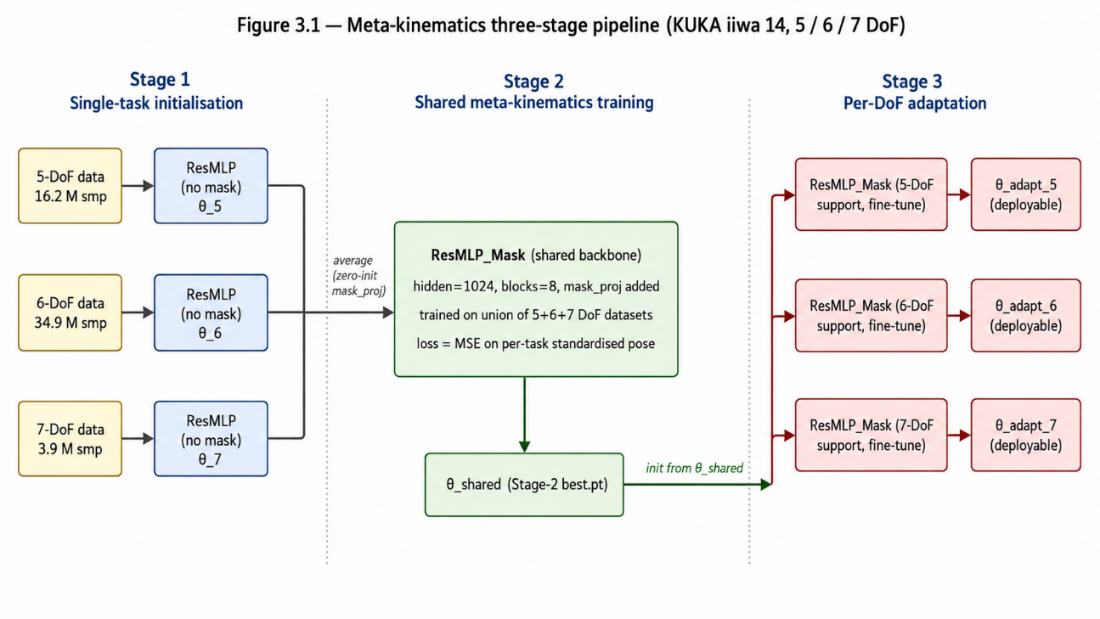
\includegraphics[width=0.9\columnwidth]{Picture/Work flow.png}
\caption{Meta-kinematics three-stage pipeline. Stage~1: per-DoF single-task FK models are trained independently on $\mathcal{D}_5$, $\mathcal{D}_6$, $\mathcal{D}_7$. Stage~2: the resulting checkpoints initialise a shared meta-kinematics model that is jointly trained on $\mathcal{D}_5 \cup \mathcal{D}_6 \cup \mathcal{D}_7$. Stage~3: the shared model is fine-tuned on each target configuration to produce a deployable per-DoF model.}
\label{fig:workflow}
\end{figure}

The KUKA iiwa~14 is configured in 5, 6, and 7~DoF by progressively fixing the distal joints while keeping the proximal ones active: joint~7 is fixed for the 6-DoF case and joints~6--7 are fixed for the 5-DoF case. All configurations share a common 11-dimensional input--output format $[q_1, \dots, q_7, x, y, z, q_w, q_x, q_y, q_z]^\top$, which allows a single model to be applied to all three tasks.

\subsection{Shared Network Architecture}
\label{sec:arch}

The shared backbone $f_\theta$ is a residual multilayer perceptron (ResMLP) with hidden dimension $1024$ and $8$ residual blocks, illustrated in Fig.~\ref{fig:arch}(a). Each residual block is Linear $\rightarrow$ ReLU $\rightarrow$ Dropout$(p{=}0.1)$ $\rightarrow$ Linear $\rightarrow$ skip-add $\rightarrow$ ReLU. The output head produces $7$ values corresponding to the standardised pose vector $[x, y, z, q_w, q_x, q_y, q_z]^\top$; predicted quaternion components are renormalised to unit norm at evaluation time. Inputs and targets are standardised per task using statistics from the training split.

To inform the network of which DoF configuration is active, the input layer combines the clamped joint vector with a learned projection of the binary task mask $\mathbf{m}_k$:
\begin{equation}
\mathbf{h}_0 = \mathrm{ReLU}\bigl(W_{\mathrm{in}}\, \tilde{\mathbf{q}} + W_{\mathrm{mask}}\, \mathbf{m}_k\bigr),
\label{eq:mask_proj}
\end{equation}
where $W_{\mathrm{mask}} \in \mathbb{R}^{1024 \times 7}$ is initialised to zero so that the network reduces to the unmasked baseline at the start of training and learns to use the mask channel only as required by the multi-task data. This is the only DoF-dependent input; no per-task heads, embeddings, or adapters are introduced, and the same backbone is reused without modification across all three configurations and all three pipeline stages, as visualised in Fig.~\ref{fig:arch}(b).

\begin{figure*}[!t]
\centering
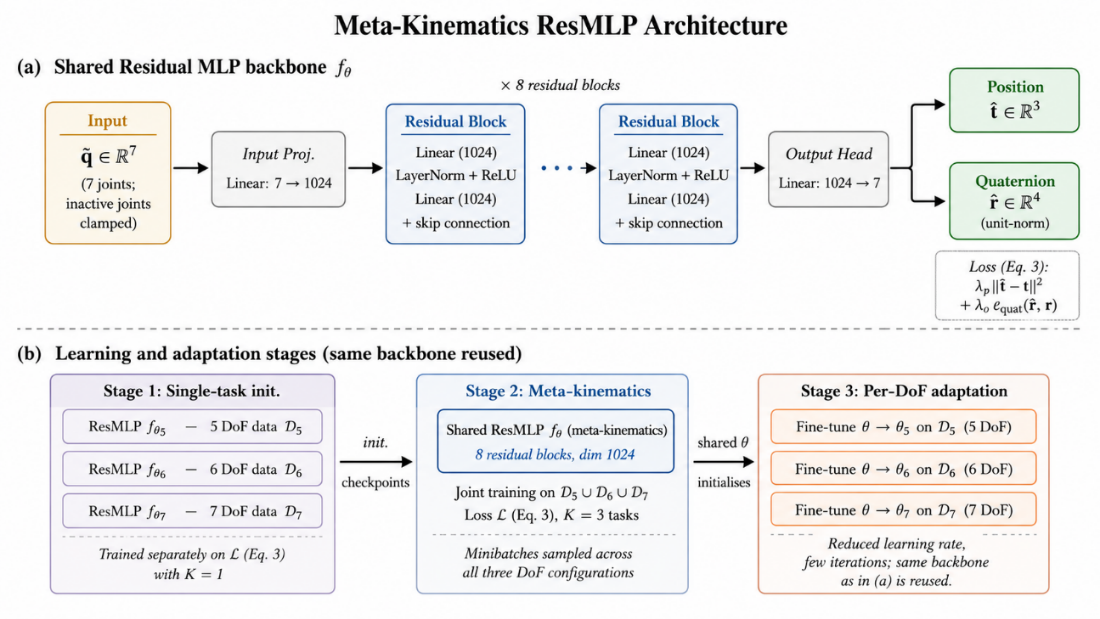
\includegraphics[width=0.7\textwidth]{Picture/meta_arch.png}
\caption{Meta-kinematics ResMLP architecture and learning stages. (a) Shared backbone $f_\theta$: the clamped joint vector $\tilde{\mathbf{q}} \in \mathbb{R}^{7}$ is projected to a hidden dimension of $1024$, summed with the learned mask projection (Eq.~\ref{eq:mask_proj}), passed through $8$ residual blocks, and mapped by the output head to the standardised pose vector $[\hat{\mathbf{t}}, \hat{\mathbf{r}}]^\top \in \mathbb{R}^{7}$. The internal block diagram is schematic; see Section~\ref{sec:arch} for the exact ResBlock structure. Stages~1 and~2 train under the regression loss~\eqref{eq:loss_reg}; Stage~3 adapts under the physical loss~\eqref{eq:loss_adapt}. (b) The same backbone is reused in all three methodology stages: per-configuration single-task initialisation (Stage~1), joint meta-kinematics training on $\mathcal{D}_5 \cup \mathcal{D}_6 \cup \mathcal{D}_7$ (Stage~2), and short per-DoF fine-tuning (Stage~3).}
\label{fig:arch}
\end{figure*}

\subsection{Meta-Kinematics Learning and Adaptation}
\label{sec:learning}

The framework is trained and deployed in three stages, summarised in Algorithm~\ref{alg:metakin}. \textbf{Stage~1 (single-task initialisation):} a separate ResMLP is trained for each $\mathcal{D}_k$ under the regression loss~\eqref{eq:loss_reg}; these models serve as task-specific baselines and as the source of strong initialisation checkpoints. \textbf{Stage~2 (shared meta-kinematics training):} the Stage~1 checkpoints are merged to seed a single shared model, which is then trained on $\mathcal{D}_5 \cup \mathcal{D}_6 \cup \mathcal{D}_7$ under the same loss~\eqref{eq:loss_reg}; at every step a task $\tau_k$ is drawn uniformly at random and a minibatch is sampled from $\mathcal{D}_k$, so that the model is pushed to explain all three configurations with a single set of parameters. \textbf{Stage~3 (per-DoF adaptation):} starting from the shared $\theta$, a short fine-tune on each target dataset using the physical objective~\eqref{eq:loss_adapt} with a reduced learning rate and $N_3 \ll N_1$ steps yields the deployable per-configuration model $\theta_k$. The $\ell_2$-to-init term in~\eqref{eq:loss_adapt} prevents adaptation from drifting too far from the shared prior.

\begin{algorithm}[!t]
\caption{Meta-Kinematics Training and Adaptation}
\label{alg:metakin}
\KwIn{Datasets $\{\mathcal{D}_k\}_{k=1}^{K}$ for DoF configurations $\{\tau_k\}_{k=1}^{K}$ with masks $\{\mathbf{m}_k\}_{k=1}^{K}$; loss weights $\lambda_p, \lambda_o, \lambda_{\mathrm{reg}}$; learning rates $\eta_1, \eta_2, \eta_3$; iteration counts $N_1, N_2, N_3$.}
\KwOut{Shared model $\theta$ and per-DoF adapted models $\{\theta_k\}_{k=1}^{K}$.}
\BlankLine
\textbf{Stage~1: Single-task initialisation}\\
\For{$k = 1, \dots, K$}{
    Initialise $\theta_k^{(0)}$ randomly\;
    Train ResMLP on $\mathcal{D}_k$ for $N_1$ epochs with loss~\eqref{eq:loss_reg} and learning rate $\eta_1$, yielding checkpoint $\theta_k^{(1)}$\;
}
\textbf{Stage~2: Shared meta-kinematics training}\\
Initialise $\theta \leftarrow \mathrm{merge}(\theta_1^{(1)}, \dots, \theta_K^{(1)})$\;
\For{$t = 1, \dots, N_2$}{
    Sample task $k \sim \mathrm{Uniform}(\{1,\dots,K\})$\;
    Sample minibatch $B \sim \mathcal{D}_k$\;
    Compute $\mathcal{L}_{\mathrm{reg}}(\theta)$ from~\eqref{eq:loss_reg} on $B$ with mask $\mathbf{m}_k$\;
    Update $\theta$ by Adam with learning rate $\eta_2$\;
}
\textbf{Stage~3: Per-DoF adaptation}\\
\For{$k = 1, \dots, K$}{
    Initialise $\theta_k \leftarrow \theta$\;
    Fine-tune $\theta_k$ on $\mathcal{D}_k$ for $N_3$ steps using loss~\eqref{eq:loss_adapt} and learning rate $\eta_3 \ll \eta_2$\;
}
\end{algorithm}

Evaluation uses position error in millimetres, reported as pose root-mean-square error (RMSE), and orientation error in degrees, computed from quaternion differences. Wall-clock training time is also recorded so that the cost of training per-configuration models from scratch can be compared with the much shorter cost of adapting from the shared meta-model.

\section{Experimental Results and Discussion}
\label{sec:exp}

\subsection{Experimental Setup}
\label{sec:setup}

\textbf{Datasets.}
Datasets were generated in Isaac Lab (Fig.~\ref{fig:sim}) by sampling joint configurations within a restricted workspace region rather than over the full mechanical joint limits, in order to focus on a practically relevant part of the configuration space. The sampling step sizes were $8^\circ$ for 5~DoF, $12^\circ$ for 6~DoF, and $15^\circ$ for 7~DoF, with each single-task dataset capped at $15$ million samples (Table~\ref{tab:dataset}). Each dataset is split $70/10/20$ into training, validation, and held-out test partitions, and all reported metrics are computed on the held-out test split.

\begin{figure}[!t]
\centering
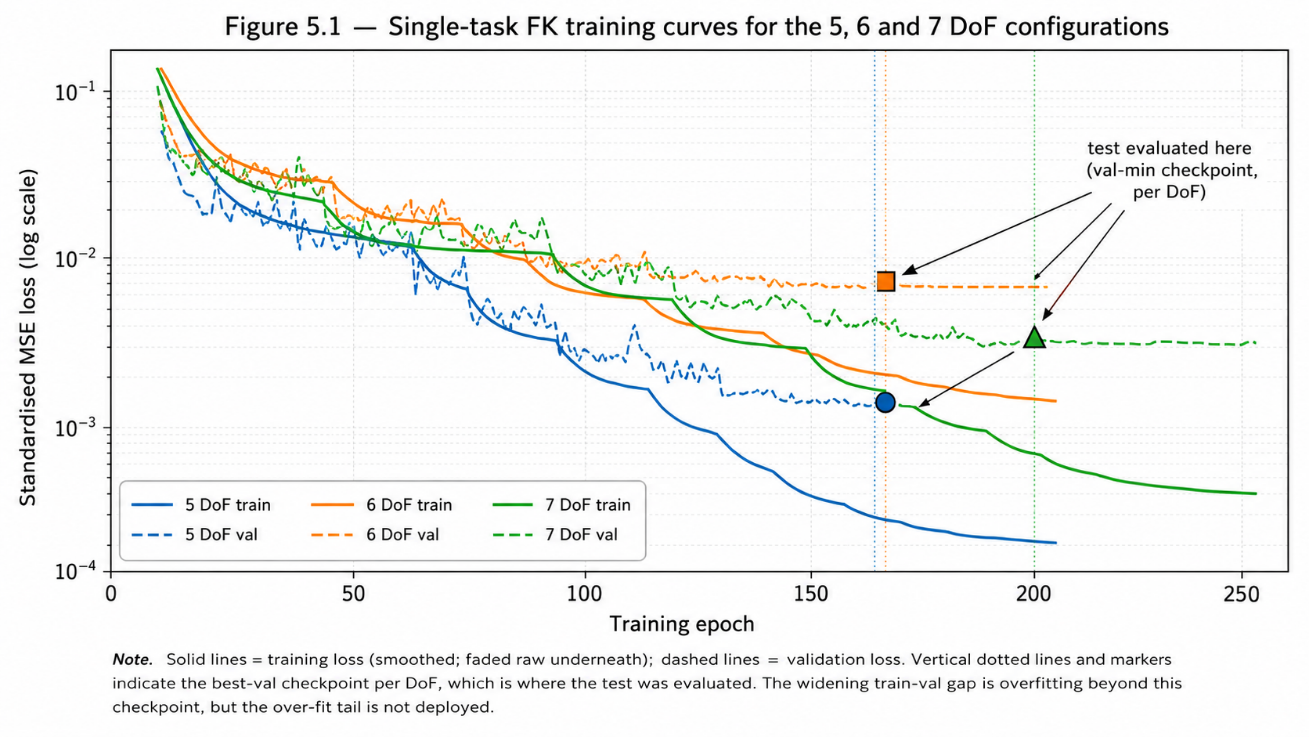
\includegraphics[width=0.9\columnwidth]{Picture/Isaac_lab.png}
\caption{Isaac Lab simulation environment used to generate the meta-kinematics datasets. The KUKA iiwa~14 (centre) is sampled across the restricted workspace region using the per-DoF step sizes of Table~\ref{tab:dataset}. The right-hand panel shows the live joint-state read-out (joint positions, velocities and torques) used to log $\mathbf{q}$ alongside the corresponding end-effector pose $\mathbf{p}$ obtained from Isaac Lab's analytical solver, which serves as ground truth.}
\label{fig:sim}
\end{figure}

\begin{table}[!t]
\renewcommand{\arraystretch}{1.2}
\caption{Dataset configuration for single-task forward kinematics.}
\label{tab:dataset}
\centering
\begin{tabular}{lccc}
\toprule
Configuration & Active Joints & Sampling Step & Sample Cap \\
\midrule
5~DoF & 1--5 & $8^\circ$  & 15M \\
6~DoF & 1--6 & $12^\circ$ & 15M \\
7~DoF & 1--7 & $15^\circ$ & 15M \\
\bottomrule
\end{tabular}
\end{table}

\textbf{Implementation and hardware.}
All models were implemented in PyTorch~2.x and trained on a single workstation with an Intel Core i9-13980HX CPU, $32$\,GB of system memory, and an NVIDIA GeForce RTX~4080 Laptop GPU ($12$\,GB). Mixed-precision (FP16) training was used. The best checkpoint by validation loss was retained for evaluation.

\textbf{Hyperparameters.}
The training hyperparameters for the three stages are summarised in Table~\ref{tab:hparams}.

\textbf{Baselines.}
Two reference points are evaluated alongside the proposed adapted meta-kinematics model: (i) a \textbf{single-task ResMLP}, trained per-configuration from scratch, which is the strongest direct learning-based FK baseline within our setting and matches the backbone used by the meta-kinematics model; and (ii) the \textbf{shared meta-kinematics model} (\emph{no adaptation}), evaluated on each configuration using the same set of parameters $\theta$. The proposed \textbf{adapted meta-kinematics model} (Stage~3 output, $\theta_k$) is then compared against both. Numbers reported in this draft are single-run point estimates; a multi-seed evaluation and an additional plain-MLP baseline representative of earlier learning-based FK studies~\cite{duka2014,koker2004} are deferred to the journal extension.

\begin{table}[!t]
\renewcommand{\arraystretch}{1.05}
\caption{Stage-structured training hyperparameters. Architectural settings are shared across stages. Loss-weight values $\lambda_p$, $\lambda_o$, $\lambda_{\mathrm{reg}}$ apply only to Stage~3 (Eq.~\ref{eq:loss_adapt}); Stages~1 and~2 use the unweighted regression loss in~\eqref{eq:loss_reg}. All stages use Adam ($\beta_1=0.9$, $\beta_2=0.999$) and gradient clipping at $1.0$.}
\label{tab:hparams}
\centering
\footnotesize
\begin{tabular}{ll}
\toprule
\multicolumn{2}{l}{\textit{Architecture (shared)}} \\
\midrule
Hidden dim. / residual blocks & $1024$ / $8$ \\
Activation; per-block dropout & ReLU; $0.1$ \\
Mask projection $W_{\mathrm{mask}}$ & zero-initialised, $\mathbb{R}^{1024 \times 7}$ \\
\midrule
\multicolumn{2}{l}{\textit{Stage~1 — single-task initialisation}} \\
\midrule
Learning rate $\eta_1$, weight decay & $5\times10^{-4}$, $1\times10^{-5}$ \\
Schedule & ReduceLROnPlateau ($\gamma=0.5$, patience $10$) \\
Batch size; iterations $N_1$ & $4096$; $200$ epochs \\
\midrule
\multicolumn{2}{l}{\textit{Stage~2 — shared meta-kinematics training}} \\
\midrule
Learning rate $\eta_2$ & $3\times10^{-4}$ \\
Schedule & cosine, warmup $2000$ steps, $\eta_{\min}=10^{-5}$ \\
Batch (per task); iterations $N_2$ & $4096$; $1{,}000{,}000$ steps \\
Task sampling & uniform over $\{5, 6, 7\}$~DoF per step \\
\midrule
\multicolumn{2}{l}{\textit{Stage~3 — per-DoF adaptation}} \\
\midrule
Learning rate $\eta_3$ ($\varepsilon=10^{-7}$) & $1\times10^{-5}$ (constant) \\
Batch size; iterations $N_3$ & $512$; $10{,}000$ steps \\
Loss weights $(\lambda_p, \lambda_o, \lambda_{\mathrm{reg}})$ & $(1.0,\, 0.1,\, 1\times10^{-6})$ \\
\bottomrule
\end{tabular}
\end{table}

\subsection{Meta-Kinematics Evaluation}
\label{sec:results}

\textbf{Training behaviour.}
Validation-loss curves for the single-task and shared meta-kinematics models are shown in Fig.~\ref{fig:curves}. The single-task ResMLPs converged smoothly for all three DoF settings (Fig.~\ref{fig:single_curve}), and the shared meta-kinematics model (Fig.~\ref{fig:multi_curve}) trained stably from the merged single-task initialisation, confirming that the shared backbone has enough capacity to represent all three configurations simultaneously.

\begin{figure}[!t]
\centering
\subfloat[Single-task FK validation loss vs.\ epoch for the 5, 6, and 7~DoF ResMLPs.]{
    \begin{tikzpicture}
    \node[anchor=south west, inner sep=0] (img) at (0,0)
        {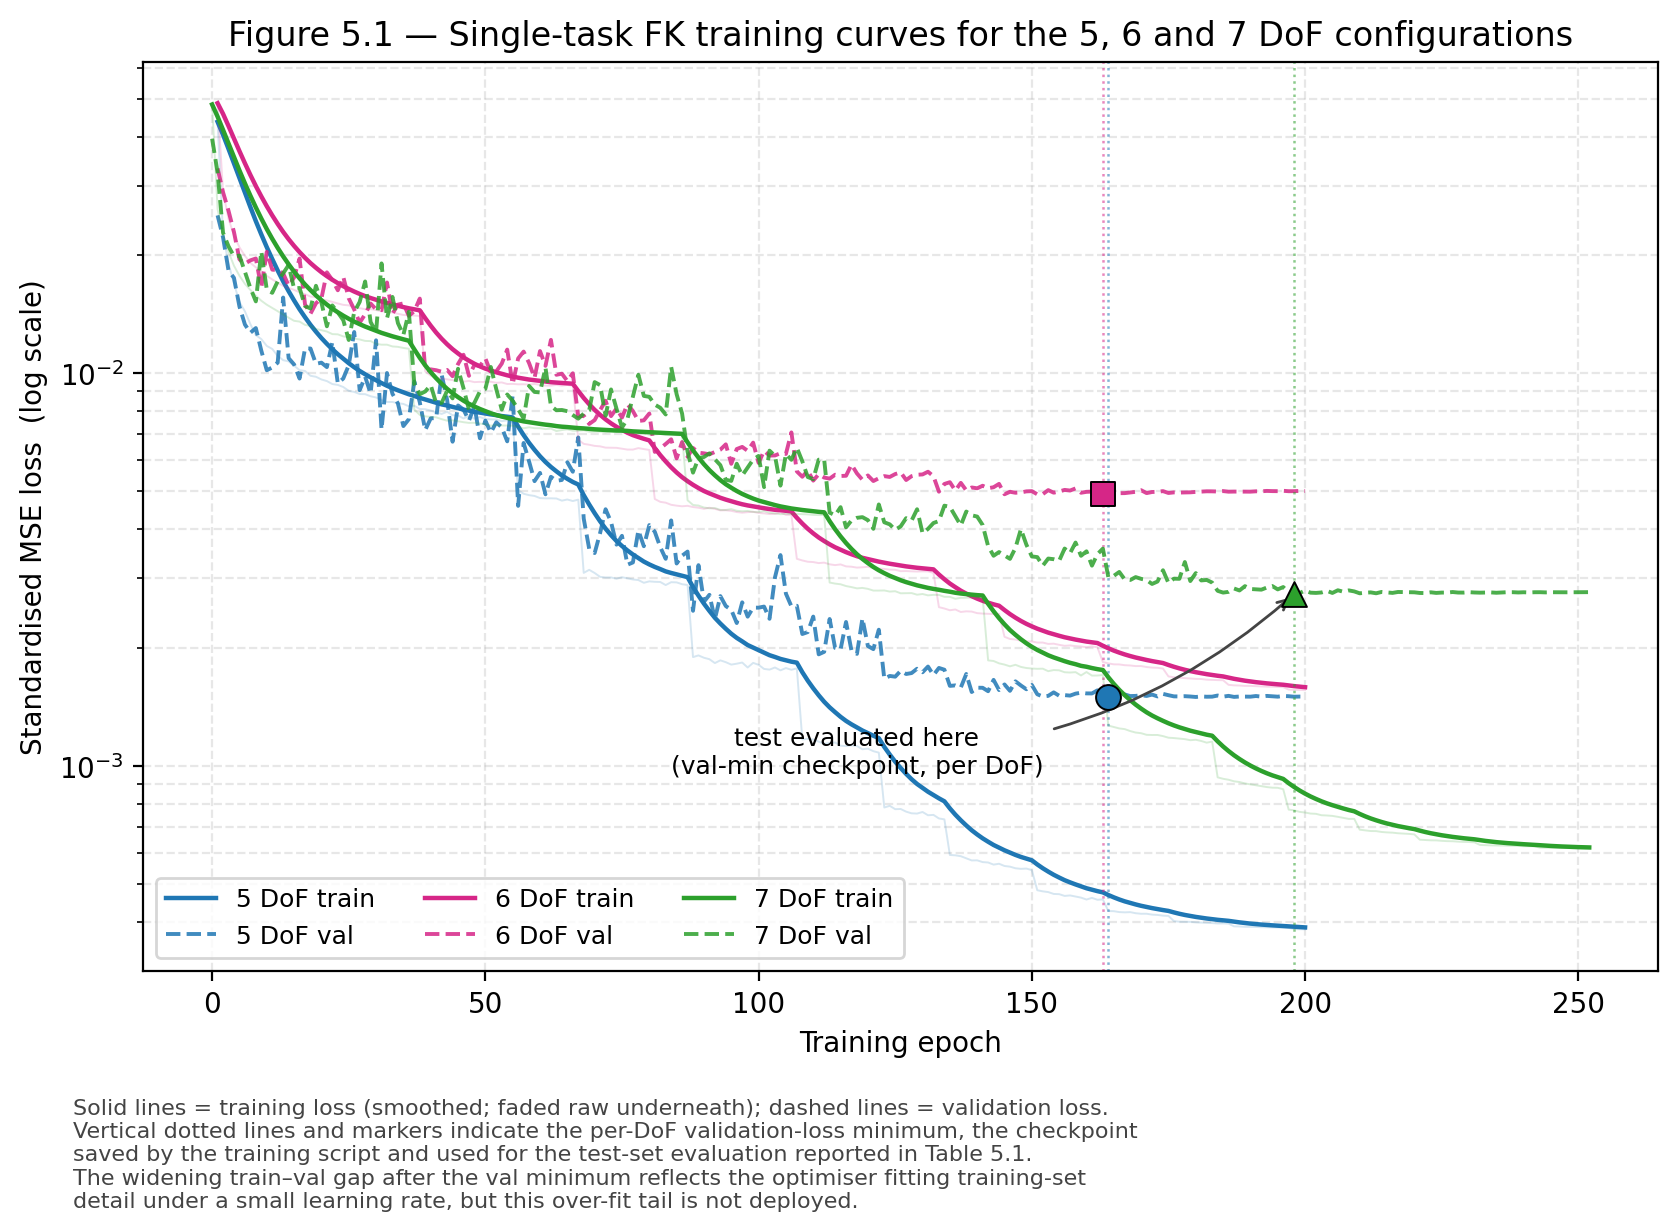
\includegraphics[width=0.85\columnwidth]{Picture/single_curve.png}};
    \begin{scope}[x={(img.south east)}, y={(img.north west)}]
        \node[anchor=north, font=\footnotesize] at (0.55, -0.02) {Epoch};
        \node[anchor=south, rotate=90, font=\footnotesize] at (-0.04, 0.5) {Validation loss};
    \end{scope}
    \end{tikzpicture}
    \label{fig:single_curve}
}\\[6pt]
\subfloat[Shared meta-kinematics validation loss vs.\ training step.]{
    \begin{tikzpicture}
    \node[anchor=south west, inner sep=0] (img) at (0,0)
        {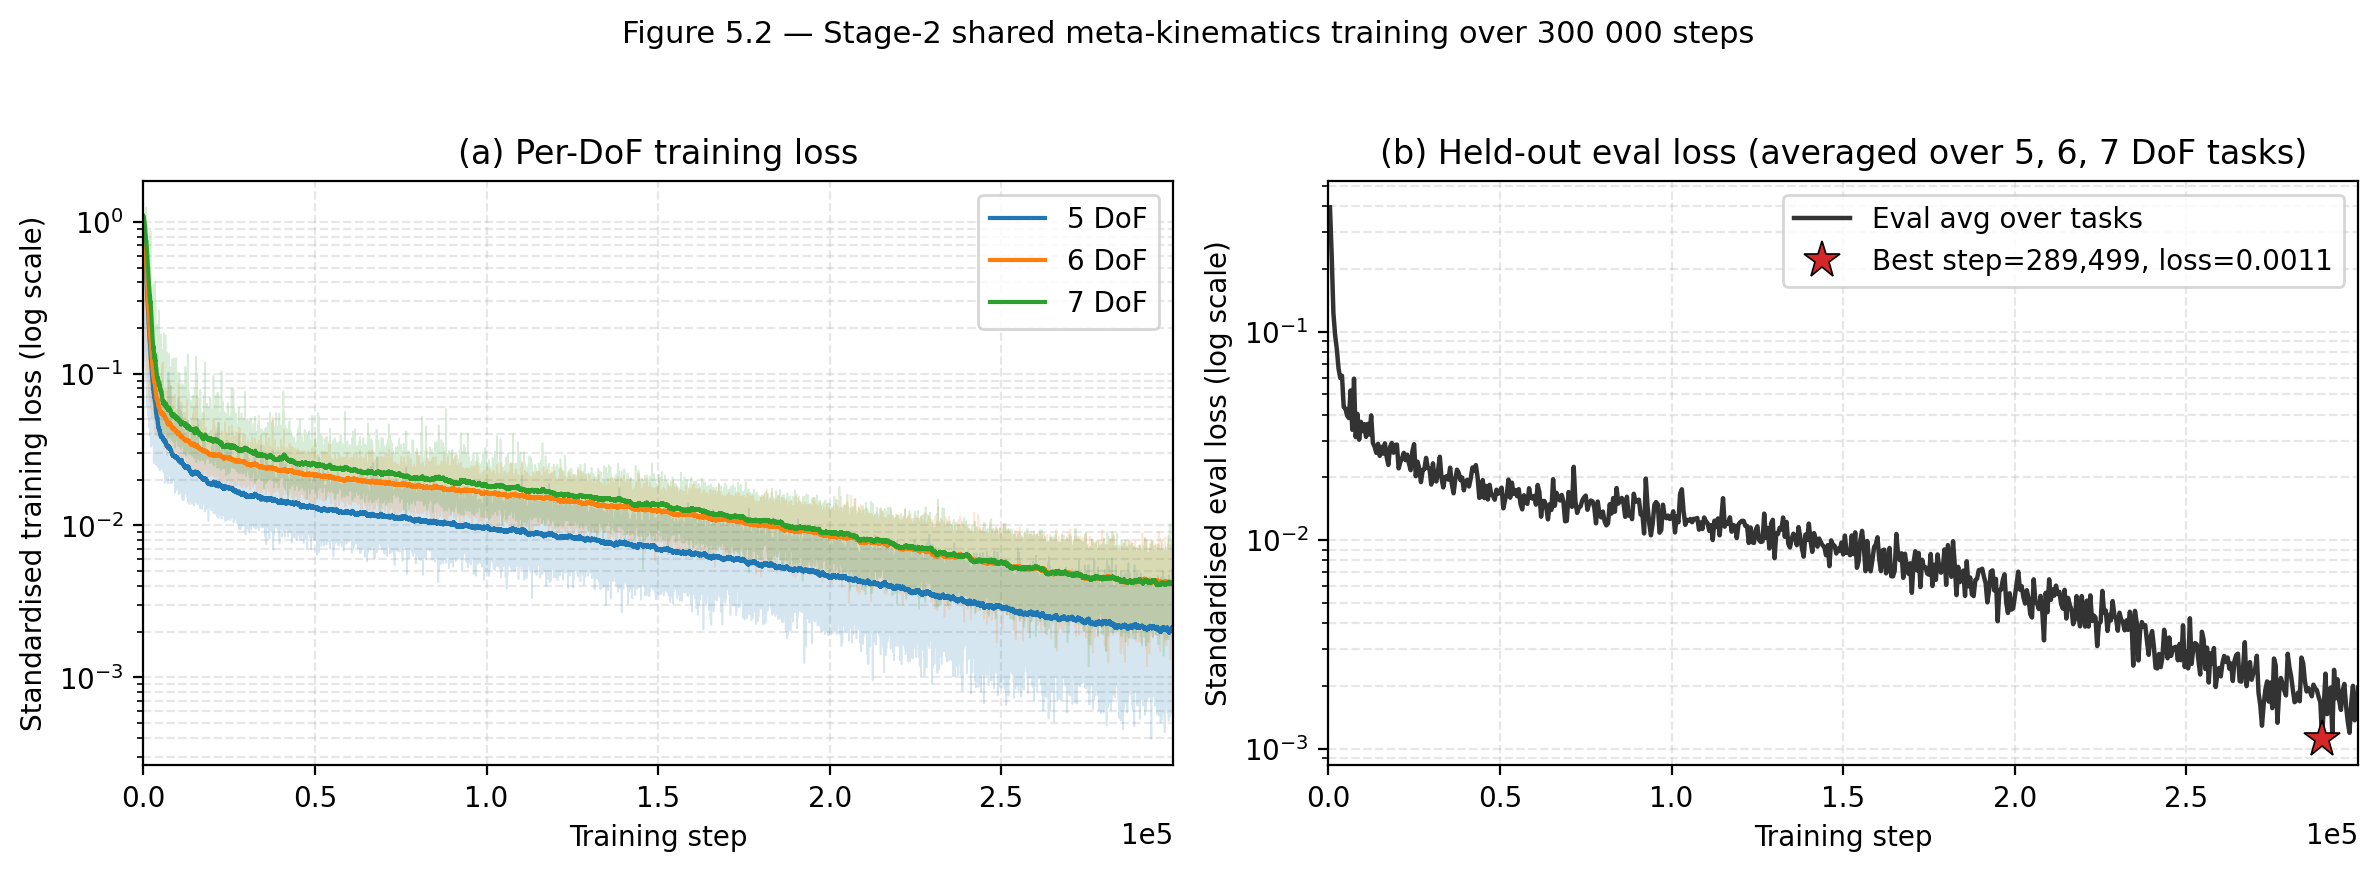
\includegraphics[width=0.85\columnwidth]{Picture/multi_task.png}};
    \begin{scope}[x={(img.south east)}, y={(img.north west)}]
        \node[anchor=north, font=\footnotesize] at (0.55, -0.02) {Training step};
        \node[anchor=south, rotate=90, font=\footnotesize] at (-0.04, 0.5) {Validation loss};
    \end{scope}
    \end{tikzpicture}
    \label{fig:multi_curve}
}
\caption{Training behaviour of the forward-kinematics models. Both panels plot validation loss (the regression loss~\eqref{eq:loss_reg} on the standardised pose vector); the horizontal axis denotes training epochs in (a) and total training steps in (b).}
\label{fig:curves}
\end{figure}

\textbf{Accuracy.}
Table~\ref{tab:results} reports the position and orientation errors of the three model variants across the 5, 6, and 7~DoF configurations. Position errors are in millimetres so that practically meaningful differences are easier to read.

\begin{table}[!t]
\renewcommand{\arraystretch}{1.15}
\caption{Forward-kinematics accuracy on the held-out test split. Position error is pose RMSE in millimetres; orientation error is the angular error in degrees, computed from quaternion differences. Single-run point estimates; best per row in \textbf{bold}.}
\label{tab:results}
\centering
\footnotesize
\begin{tabular}{llccc}
\toprule
Config. & Metric & \makecell{Single-Task\\ResMLP} & \makecell{Shared\\Meta-Kin.} & \makecell{Adapted\\Meta-Kin.} \\
\midrule
\multirow{2}{*}{5~DoF}
& Pos.\ (mm)        & $9.30$  & $6.80$  & $\mathbf{6.20}$ \\
& Ori.\ ($^\circ$)  & $1.2039$ & $0.9096$ & $\mathbf{0.8036}$ \\
\midrule
\multirow{2}{*}{6~DoF}
& Pos.\ (mm)        & $11.00$ & $9.20$  & $\mathbf{9.00}$ \\
& Ori.\ ($^\circ$)  & $1.7136$ & $1.3689$ & $\mathbf{1.3385}$ \\
\midrule
\multirow{2}{*}{7~DoF}
& Pos.\ (mm)        & $10.10$ & $10.90$ & $\mathbf{9.90}$ \\
& Ori.\ ($^\circ$)  & $2.0853$ & $1.9953$ & $\mathbf{1.7104}$ \\
\bottomrule
\end{tabular}
\end{table}

\textbf{Training cost.}
Table~\ref{tab:time} reports wall-clock training time on the rig of Section~\ref{sec:setup}. The shared meta-kinematics model is trained \emph{once} for all three configurations and its cost is therefore amortised across the per-DoF adaptations rather than being incurred per task.

\begin{table}[!t]
\renewcommand{\arraystretch}{1.15}
\caption{Wall-clock training time (hours) on the rig of Section~\ref{sec:setup}. The shared meta-kinematics model is trained \emph{once} across all three configurations; its cost is reported on a single row spanning the three columns. The relative reduction is the percentage decrease of the adapted meta-kinematics time over the corresponding single-task ResMLP. Single-run point estimates.}
\label{tab:time}
\centering
\footnotesize
\begin{tabular}{lccc}
\toprule
Stage / Variant & 5~DoF & 6~DoF & 7~DoF \\
\midrule
Single-Task ResMLP & $1.873$ & $4.973$ & $22.120$ \\
Shared Meta-Kin.\ (once for all 3) & \multicolumn{3}{c}{$1.159$} \\
Adapted Meta-Kin.\ (per DoF) & $\mathbf{0.365}$ & $\mathbf{0.363}$ & $\mathbf{0.111}$ \\
\midrule
Reduction over Single-Task & $-80.5\%$ & $-92.7\%$ & $-99.5\%$ \\
\bottomrule
\end{tabular}
\end{table}

Three advantages of the meta-kinematics framework are evident from Tables~\ref{tab:results} and~\ref{tab:time}. First, transferable kinematic structure is captured \emph{without} per-task training: the shared meta-model already matches the single-task ResMLP baselines in the 5 and 6~DoF cases, and remains within a small margin in the 7~DoF case, while using a single set of parameters rather than three. Second, per-DoF adaptation consistently improves over both the shared meta-model and the single-task ResMLP baselines, yielding the lowest position and orientation errors across all three configurations; in the 7~DoF case, for example, the adapted meta-model reduces orientation error by $18.0\%$ relative to the single-task baseline (from $2.0853^\circ$ to $1.7104^\circ$). Third, the adaptation stage requires substantially less training time than single-task training from scratch: $-80.5\%$ in the 5~DoF case, $-92.7\%$ in the 6~DoF case, and $-99.5\%$ in the 7~DoF case, while maintaining or improving accuracy.

\subsection{Discussion}

The pattern in Table~\ref{tab:results} supports the interpretation that the shared meta-model has learned transferable forward-kinematics knowledge rather than three independent mappings represented within a single network. If the shared parameters represented only a compromise between the three tasks, per-DoF adaptation would, at best, recover the single-task baseline. Instead, adaptation improves over the baseline in every configuration, which indicates that the fine-tuning stage exploits a useful prior established during shared training.

This advantage is most pronounced in the 7~DoF case. Training a single-task 7~DoF model is considerably more costly than the 5 or 6~DoF cases because the configuration space is larger, yet the adapted meta-model attains improved accuracy at a small fraction of the training cost. This is the scenario in which meta-kinematics offers the greatest practical benefit: when the target configuration is expensive to train from scratch, the one-off cost of training a shared meta-model is rapidly amortised across successive adaptations.

\textbf{Limitations.}
The study is limited to simulation; real-robot validation is required to assess transfer under calibration error, sensing noise, and simulator-to-hardware mismatch. The framework is also evaluated on a single manipulator, so the extent to which the meta-kinematics representation generalises across robot families remains open. The accuracy and training-time figures are single-run point estimates; a multi-seed evaluation with mean~$\pm$~standard deviation, together with an additional plain-MLP baseline representative of earlier learning-based FK studies~\cite{duka2014,koker2004}, is left for the journal extension. Finally, the formulation assumes that inactive joints take fixed, known values.

\section{Conclusion and Future Work}
\label{sec:conclusion}

This paper has presented a meta-kinematics framework that learns a single forward-kinematics model across multiple DoF configurations of the same robot and adapts it efficiently to each target configuration. On the KUKA iiwa~14 in 5, 6, and 7~DoF settings, the shared meta-model captured transferable kinematic structure, and short per-DoF adaptation matched or exceeded the single-task ResMLP baselines while reducing training time by $80.5\%$, $92.7\%$, and $99.5\%$, respectively, suggesting that meta-kinematics is a practical approach for the efficient deployment of learned forward-kinematics models across related configurations. Future work will extend the framework to (i)~inverse kinematics, where solution multi-modality raises new challenges for the meta-learning formulation; (ii)~physical-robot evaluation on the KUKA iiwa~14 with sim-to-real adaptation; and (iii)~cross-robot meta-kinematics, training the shared backbone across different manipulator families to test how much of the learned structure is robot-specific versus generic to articulated rigid-body chains.

\section*{Acknowledgment}
The authors thank the project supervisor for guidance throughout this work.

\begin{thebibliography}{9}
\setlength{\itemsep}{2pt plus 1pt}

\bibitem{siciliano2009}
B. Siciliano, L. Sciavicco, L. Villani, and G. Oriolo, \emph{Robotics: Modelling, Planning and Control}. London, U.K.: Springer, 2009.

\bibitem{duka2014}
A. Duka, ``Neural network based inverse kinematics solution for trajectory tracking of a robotic arm,'' \emph{Procedia Technology}, vol. 12, pp. 20--27, 2014.

\bibitem{koker2004}
R. K{\"o}ker, C. {\"O}z, T. {\c{C}}akar, and H. Ekiz, ``A study of neural network based inverse kinematics solution for a three-joint robot,'' \emph{Robotics and Autonomous Systems}, vol. 49, no. 3--4, pp. 227--234, 2004.

\bibitem{diprasetya2025}
M. R. Diprasetya, J. P{\"o}ppelbaum, and A. Schwung, ``KineNN: Kinematic neural network for inverse model policy based on homogeneous transformation matrix and dual quaternion,'' \emph{Robotics and Computer-Integrated Manufacturing}, vol. 94, p. 102945, 2025.

\bibitem{devin2017}
C. Devin, A. Gupta, T. Darrell, P. Abbeel, and S. Levine, ``Learning modular neural network policies for multi-task and multi-robot transfer,'' in \emph{Proc. IEEE Int. Conf. Robotics and Automation}, 2017, pp. 2169--2176.

\bibitem{chen2018}
T. Chen, A. Murali, and A. Gupta, ``Hardware conditioned policies for multi-robot transfer learning,'' in \emph{Advances in Neural Information Processing Systems}, 2018, pp. 9355--9366.

\bibitem{ghadirzadeh2021}
A. Ghadirzadeh, X. Chen, P. Poklukar, C. Finn, M. Bj{\"o}rkman, and D. Kragic, ``Bayesian meta-learning for few-shot policy adaptation across robotic platforms,'' in \emph{Proc. IEEE/RSJ Int. Conf. Intelligent Robots and Systems}, 2021, pp. 1277--1284.

\bibitem{byravan2017}
A. Byravan and D. Fox, ``SE3-Nets: Learning rigid body motion using deep neural networks,'' in \emph{Proc. IEEE Int. Conf. Robotics and Automation}, 2017, pp. 173--180.

\bibitem{byravan2018}
A. Byravan, F. Leeb, F. Meier, and D. Fox, ``SE3-Pose-Nets: Structured deep dynamics models for visuomotor control,'' in \emph{Proc. IEEE Int. Conf. Robotics and Automation}, 2018, pp. 3339--3346.

\end{thebibliography}

\end{document}